

% Place an \includeonly here to only compile certain parts
% e.g.: \includeonly{title,chapter-first,references}

\documentclass[]{article}\usepackage[]{graphicx}\usepackage[]{color}
%% maxwidth is the original width if it is less than linewidth
%% otherwise use linewidth (to make sure the graphics do not exceed the margin)
\makeatletter
\def\maxwidth{ %
  \ifdim\Gin@nat@width>\linewidth
    \linewidth
  \else
    \Gin@nat@width
  \fi
}
\makeatother

\definecolor{fgcolor}{rgb}{0.345, 0.345, 0.345}
\newcommand{\hlnum}[1]{\textcolor[rgb]{0.686,0.059,0.569}{#1}}%
\newcommand{\hlstr}[1]{\textcolor[rgb]{0.192,0.494,0.8}{#1}}%
\newcommand{\hlcom}[1]{\textcolor[rgb]{0.678,0.584,0.686}{\textit{#1}}}%
\newcommand{\hlopt}[1]{\textcolor[rgb]{0,0,0}{#1}}%
\newcommand{\hlstd}[1]{\textcolor[rgb]{0.345,0.345,0.345}{#1}}%
\newcommand{\hlkwa}[1]{\textcolor[rgb]{0.161,0.373,0.58}{\textbf{#1}}}%
\newcommand{\hlkwb}[1]{\textcolor[rgb]{0.69,0.353,0.396}{#1}}%
\newcommand{\hlkwc}[1]{\textcolor[rgb]{0.333,0.667,0.333}{#1}}%
\newcommand{\hlkwd}[1]{\textcolor[rgb]{0.737,0.353,0.396}{\textbf{#1}}}%

\usepackage{framed}
\makeatletter
\newenvironment{kframe}{%
 \def\at@end@of@kframe{}%
 \ifinner\ifhmode%
  \def\at@end@of@kframe{\end{minipage}}%
  \begin{minipage}{\columnwidth}%
 \fi\fi%
 \def\FrameCommand##1{\hskip\@totalleftmargin \hskip-\fboxsep
 \colorbox{shadecolor}{##1}\hskip-\fboxsep
     % There is no \\@totalrightmargin, so:
     \hskip-\linewidth \hskip-\@totalleftmargin \hskip\columnwidth}%
 \MakeFramed {\advance\hsize-\width
   \@totalleftmargin\z@ \linewidth\hsize
   \@setminipage}}%
 {\par\unskip\endMakeFramed%
 \at@end@of@kframe}
\makeatother

\definecolor{shadecolor}{rgb}{.97, .97, .97}
\definecolor{messagecolor}{rgb}{0, 0, 0}
\definecolor{warningcolor}{rgb}{1, 0, 1}
\definecolor{errorcolor}{rgb}{1, 0, 0}
\newenvironment{knitrout}{}{} % an empty environment to be redefined in TeX

\usepackage{alltt}
\usepackage[T1]{fontenc}
\usepackage{titlesec}           % For keeping section/chapter titles
                                % single-spaced
\usepackage{blindtext}
\usepackage[margin=1.25in]{geometry}
\usepackage{url}
\urlstyle{sf}

\usepackage{jrnoldStats}

\usepackage[newfloat]{minted}

\usepackage{subcaption}
\usepackage{enumitem}

\usepackage{tikz}

\usepackage[all]{nowidow}

\usepackage[]{xcolor}
\definecolor{light-gray}{gray}{0.66}
\definecolor{dkred}{rgb}{0.5,0,0}
\definecolor{dkblue}{rgb}{0,0,0.5}

\usepackage{hyperref}
\hypersetup{
  pdftitle={Three Essays on Conflict and Financial Markets, and Political Methodology},
  pdfauthor={Jeffrey B. Arnold},
  pdfkeywords={},
  %% Colors from jss.cls (Journal of statistical software)
  colorlinks = true,
  linkcolor=dkblue,          % color of internal links
  citecolor=dkblue,        % color of links to bibliography
  filecolor=dkred,      % color of file links
  urlcolor=dkred,           % color of external links
}


\usepackage{fontspec,xltxtra,xunicode}
\defaultfontfeatures{Mapping=tex-text}
\setmainfont[Ligatures=TeX]{Linux Libertine O}
\setsansfont[Ligatures=TeX, Scale=MatchLowercase]{Source Sans Pro}
\setmonofont[Scale=MatchLowercase]{Source Code Pro}
\usepackage[math-style=TeX]{unicode-math}
\setmathfont{xits-math.otf}


% Misc
\newcommand{\email}[1]{\href{mailto:#1}{\normalfont\texttt{#1}}}
\newcommand{\eg}{\textit{e.g.}\ }
\newcommand{\ie}{\textit{i.e.}\ }

% biblatex
\usepackage[style=authoryear,backend=biber,%
            backref=true,maxbibnames=10,hyperref=true,%
            dateabbrev=false,uniquename=false,backend=biber]{biblatex}
\AtEveryBibitem{\clearlist{language}}
\AtEveryBibitem{\clearlist{eprint}}
%% \DeclareFieldFormat{linked}{%
%%   \ifboolexpr{ test {\ifhyperref} and not test {\ifentrytype{online}} }
%%     {\iffieldundef{doi}
%%        {\iffieldundef{url}
%%           {\iffieldundef{isbn}
%%              {\iffieldundef{issn}
%%                 {#1}
%%                 {\href{\worldcatsearch\thefield{issn}}{#1}}}
%%              {\href{\worldcatsearch\thefield{isbn}}{#1}}}
%%           {\href{\thefieldfirstword{url}}{#1}}}
%%        {\href{http://dx.doi.org/\thefield{doi}}{#1}}}
%%     {#1}}
%% \newbibmacro{string+url}[1]{%
%%  \iffieldundef{doi}{\iffieldundef{url}{#1}{\href{\thefield{url}}{#1}}}{\href{http://dx.doi.org/\thefield{doi}}{#1}}}
\renewbibmacro{in:}{%
  \ifentrytype{article}{}{\printtext{\bibstring{in}\intitlepunct}}}


%\addbibresource{../bib/jrnold}
\bibliography{../bib/jrnold.bib}

\usepackage{placeins}

\title{Did Financial Markets Anticipate the Onset of the American Civil War?}
\author{Jeffrey B. Arnold}

\frenchspacing
\IfFileExists{upquote.sty}{\usepackage{upquote}}{}
\begin{document}

\maketitle{}

\begin{abstract}
  I estimate the market implied \textit{ex ante} probability of the onset of the American Civil War using U.S. government and state bonds.
  Surprisingly, financial markets were surprised by the Battle of Fort Sumter and the start of the war.
  Prior to Abraham Lincoln's election in November 1860, the market assigned almost no probability to a war.
  Even after the secession of several states, the week before the Battle of Fort Sumter, the market assigned a negligible probability, approximately 5\%, to war onset.
\end{abstract}


To what extent did financial markets anticipate the start of the American Civil War?
How did the market's assessment of war risk change leading up to the war?
Which events were associated with these changes?
This work answers these questions using data on the prices and yields of U.S. government and state bonds between 1855 and the start of the war in April 1861.
Three measures are used to assess the market's beliefs about the risk of war: bond yields, the spread between Northern and Southern state bonds, and the implied default probability of the bonds.
These measure show that the financial market did not anticipate the conflict, even immediately prior to the start of hostilities.
The financial market assigned a negligible probability of war prior to the election of Abraham Lincoln in 1860.
After the election, it increased its probability of war, but that probability was quite small.
Bond prices on April 13, 1861, immediately prior to news of the Battle of Fort Sumter, which started the war, reaching New York City implied only a 4.1 (3.3, 4.9) percent chance of war.%
\footnote{Interpret ``4.1 (3.3, 4.9)'' as ``mean (2.5\% quantile, 97.5\% quantile)''}

The results in this work speak to two important international relations theories: the bargaining theory of war \parencite{Fearon1995} and the capitalist peace \parencites{GartzkeLiEtAl2001a}{GartzkeLi2003}.
In rationalist theories of war, there are two fundamental explanations as to why two parties would fight a costly conflict rather than come to an agreement: private information and commitment problems \parencites{Fearon1995}{Powell2006}.
Although some progress has been made, it is notoriously difficult to test these mechanisms \parencite{Reiter2003}.
The use of financial market data may allow some progress in testing these theories.
Prices of certain assets whose payoffs are contingent on war outcomes, e.g.\ sovereign bonds, can be used as estimates of war initiation or outcome conditional on the public information available at the time.
From this, the researcher can calculate an implied probability of the occurrence of war.
This is useful because different theories of war have have different implications as to how uncertain wars are \textit{ex ante}.
Wars due to private information should be unanticipated \parencite{Gartzke1999}.
Since commitment problem wars can occur with complete information nothing requires them to be unanticipated.
%In the original formulation of a private information theory of war \parencite{Fearon1995}, 
%Other models may imply different \textit{ex ante} public information probabilities of conflict.
The point is that many models of war have implications of the \textit{ex ante} probability of war, and prices of some assets can be used to as a measure of this \textit{ex ante} probability.
Thus, financial markets may provide another means to test rationalist theories of war initiation.
Additionally, the inability of markets to assess the \textit{ex ante} probability of war casts doubt on their ability to signal to the cost of war to potential belligerents as in the capitalist peace theory.

This work contributes to an economic history literature on the reactions of financial markets to events within the American Civil War.
This includes multiple works on reactions of the financial markets on both sides and Europe to the American Civil War \parencites{Schwab1901}{Mitchell1903}{WillardGuinnaneEtAl1996}{McCandless1996}{SmithSmith1997}{BrownBurdekin2000}{Weidenmier2002}.
This work adds to that literature by analyzing the initiation of the war and by using Northern and Southern state bond data.
This work also adds to the growing international relations literature on the American Civil War, which has often been overlooked in the international relations literature as most work on civil wars focuses on civil wars after 1945 \parencites{Poast2012}{Reiter2009}.
This work employs methods similar to \textcite{HaberMitchenerOosterlinckEtAl2015}, which estimates the implied probability of victory in the American Civil War and the Chinese Civil War from bond prices.
More broadly, this work adds to the literature that analyzes the reactions of financial markets to conflict and political events.
Other works which have analyzed the responses of financial markets to conflicts include: \textcite{Bueno1990}, \textcite{Hall2004} and \textcite{Ferguson2006} (World War I), and \textcites{WaldenstromFrey2008}{WaldenstromFrey2008} (World War II).
\textcite{SchneiderTroeger2006} analyze the reactions of major stock market indices to events in Iraq, Israel, and the former Yugoslavia from 1990-2000.
\textcite{GuidolinLaFerrara2010} analyzes market reactions to militarized interstate disputes.
Several works look at reactions of markets to the Iraq War \parencites{RigobonSack2005}{LeighWolfersEtAl2003}{WolfersZitzewitz2009}.
Other works estimate response of financial markets to elections or political change \parencites{Jayachandr2006}{Herron2000}.

\section{Financial Market Prices and War Initiation}
\label{sec:risky-bond-pricing}

The objective of this work is to use the prices and yields of bonds to infer market beliefs about the \textit{ex ante} probability of war in the period leading up to the American Civil War.
As such, it is important to establish the theoretical relationship between the observed market prices and yields and the market's beliefs about war.
The price of a bond is the present discounted value of future cash flows.
Since the timely payment of these cash flows is uncertain, the price is an expectation of receiving these cash flows, given current information.
Thus the current price of a bond is a quantitative summary of investors' beliefs about future bond cash flows.
Since war can have large effects on these cash flows, the prices of those bonds are effectively predictions of war risk given current information.
To be able to use a bond, or other financial asset, to make inferences about the risk of war requires (1) that future payments from that asset are contingent on the war, either directly or indirectly, and (2) that there are no other factors affecting the future payments, or that the analyst is able to control for those factors.
This section discusses the how the data and methods used in this work address those criteria.

To the extent that a war would change investors' expectations about the timely payment of future cash flows of these bonds, changes in the yields of bonds can be used to infer changes in beliefs about the probability of war.
It is certainly case that war would influence expectations about the cash flows of the U.S. government and state bonds considered here.
A war would influence the credit of the issuers by increasing debt, decreasing revenue and possibly leading to default or inflation, and contemporary investors were aware of these risks.

For investors holding U.S. government bonds, secession and war would reduce the ability of the U.S. government to pay its debts both by reducing potential revenue due to the loss of the Southern states and increasing debt to pay war expenditures.
The revenue of the United States would be reduced by the secession of Southern states due to the loss of tax revenue. In 1860, the Southern states accounted for 25 percent of the non-slave wealth of the United States \parencite[11]{Elder1865}.%
\footnote{GDP was not invented until WWII.
  During the civil war era, the census estimates of personal and property wealth were used as a measure of the total economic activity and also explicitly used to assess the ability of the United States to repay the debt \parencites{Elder1863}{Elder1865}.
}
In January 1861, the \textit{Merchants' Magazine} wrote,
\begin{quote}
   The news [of secession] was also of a character to affect disastrously American credit, since it showed a decline of 13 per cent in United States government stocks, solely from fear of disunion, which event would reduce the States to the condition of the bankrupt, ``disorderly houses'' of South America, and leave the separate States a prey to every spoiler. \parencite[79]{HomansDana1861a}
\end{quote}
A war would also likely increase the debt of the United States due to increased military expenditure.
While the U.S. government only infrequently issued debt during the 19th century, the exception was to fund wars.
The U.S. government issued debt to fund the War of 1812 and the Mexican-American War of 1846--1848.
%% Later assessments of the ability of the United States to pay its debts often compared the current resources and debt levels of the United States to those of the United States in 1791 and 1816, and Great Britain during the Napoleonic Wars \parencites{Elder1863}[8 pp.]{BankersMagazine1862},
%% \footnote{
%%   The \textit{Annual Report Dec 1861} makes one of these comparisons,
%%   \begin{quote}
%%     The amount of the public  debt in the year 1816 was \$127,334,933 74, and in twenty years it was paid off by the people.
%%     The country, even if the loyal States only are regarded, can sustain and pay off in thirty years the debt to which rebellion now exposes us with hardly greater proportional contributions from increased and increasing resources than that debt
%% made necessary. (p. 23)
%%   \end{quote}
%% }
Although the war would continue much longer than initial estimates, even these initial estimated costs of war represented a large increase over peacetime expenditures and an increase in government debt.
The July 4, 1861 \textit{Report of the Secretary of the Treasury} estimated government expenditures of \$319 million for the 1861 fiscal year\parencite[5]{Treasury1861a}.%
\footnote{Fiscal year 1861 included the dates July 1, 1861 to June 30, 1862.} 
This represented an increase of 369\% (251 million) over the estimated expenditures from the previous years' report \parencite[6]{Treasury1860}.
The \textit{Annual Report} proposed paying for the new expenditures with 25\% taxes, 75\% new loans.%
\footnote{80 million in taxes, and 240 million in new loans \parencite[6]{Treasury1861a}.}
The Act of July 17, 1861, the first act passed by Congress to fund the war, authorized the issue of \$250 million in debt \parencite[44]{Treasury1863}, an increase of 178\% over the existing debt level at the time.%
\footnote{The debt on July 1, 1861 was 90 million \parencite[23]{Treasury1861a}.}
By comparison, the debt at the end of the War of 1816 was 127 million \parencite[29]{Elder1863} and only 49 million in debt was issued to fund the Mexican American War.%
\footnote{During the Mexican-American War, the Loans of 1846, 1847 and 1848 used to fund the war totaled \$49 million \parencite[42]{Treasury1863}.}

For Northern investors holding Southern state bonds, the immediate risk was that Southern states would would default on interest payments, which they did.
After the initiation of the war, Southern states immediately ceased interest payments to Northern creditors, starting with coupon payments due on July 1st, 1861 \parencites[947]{BankersMagazine1860}[159]{BankersMagazine1862}.
Investors almost certainly anticipated this as there was concern that the Southern states would default on their January 1861 payments: ``the decline [in the price of Virginia, Tennessee and Missouri bonds] \dots was further stimulated by the political condition of the country and doubts as to the prompt payment of interest by these States \parencite[756]{BankersMagazine1860}.''
After the initiation of the war, the concern over default on interest payments was the primary reason cited for the decline in the prices of Southern state bonds: ``These low values [prices of Southern state bonds] have partly been caused by the fear that these States will not be disposed to provide for the payment of their semi annual interest in July next \parencite[947]{BankersMagazine1860}.''
After Southern states had stopped paying interest, Northern investors almost certainly believed that as long as the war would continue, they not receive interest payments.
In November 1861, the \textit{Bankers' Magazine} wrote, ``...but faint hopes are entertained of their [Southern states] paying their interest for some years to come.'' \parencite[559]{BankersMagazine1862}
After the war, most Southern states repaid the debt issued before the war, but defaulted on all debt issued while part of the Confederacy and some defaulted on debt issued by reconstruction governments \parencites{Randolph1931}{Ratchford1941}.
How the Southern state governments would have handled the repayment of debt if the Confederacy had won the war is unclear.
At best, the Southern states would resume paying interest and principal soon after the end of the war, possibly with compensation for missed payments.
At worst, they would completely default on their obligations to Northern creditors.
That the prices of Southern state bonds never came close to zero, suggests that investors' beliefs put some probability on those states being reincorporated into the United States, or that the Southern states would repay their debts after the war, even in the event of a Confederate victory.
An additional means by which the war could affect the creditworthiness of Southern states is through the cost of the war.
An extended war would result in both more debt issued by Southern states to pay for the war, and destruction of human and physical capital in those states, both of which would affect the debt servicing ability of the Southern states.
Thus, holders of Southern state bonds were particularly exposed to war risk, and almost certain to suffer losses immediately at the onset of a conflict.

In order to be able to confidently make inferences about the risk of war given bond prices, alternative effects on bond prices and yields need to be controlled for.
This work accounts for these other effects in several ways.
First, it focuses on the period close to the start of the war.
Changes in the bond price are more likely to be due to changes in war risk the closer in time to the start of the war.
For example, a large price change in bond prices the week before before the Battle of Fort Sumter is more likely to be related to changes in the expectation of a war than a change in bond prices in 1850.
Second, multiple measures are used.
Third, within each of those measures multiple bonds are used.
This averages over idiosyncratic shocks to each bond.
The south-north yield spread also controls for shocks which effect all bonds.

Although U.S. government and state bonds were not prediction markets of the onset of war, since the expected payment of their future cash flows would be heavily influenced by the onset of war, they can be used to measure investors' beliefs about the onset of war.

\section{Data}
\label{sec:data}

The financial market data used in this work are the prices and yields of U.S. government and state bonds traded in New York City between 1855 and 1861.%
\footnote{
  The data used here is available at \url{https://github.com/jrnold/civil_war_era_findata}.
  The particular dataset used in this section is \href{https://github.com/jrnold/civil_war_era_findata/blob/master/data/bankers_magazine_govt_state_loans_yields_2.csv}{bankers\_magazine\_govt\_state\_loans\_yields\_2.csv}.
}
The data consist of bonds issued by five Southern states (Georgia, Louisiana, North Carolina, Tennessee, and Virginia), two Border states (Kentucky, Missouri), three Northern States (Indiana, Ohio, and Pennsylvania), and two bonds issued by the U.S. government (Sixes of 1868, Fives of 1874).%
\footnote{In the financial jargon of that era, ``Fives'' or ``5's'' refers to coupon bonds paying 5 percent interest, and ``Sixes'' or ``6's'' to coupon bonds paying 6 percent interest.}
The set of bonds included here are those which were regularly quoted in \textit{The Bankers' Magazine and Statistical Register}, a monthly business magazine.%
\footnote{After constructing this data I became aware that \textcite{DwyerHaferWeber1999} constructed a dataset of state bonds from the source.
  The data used here expands upon the price data presented in the original source, by matching each quoted price in the source with metadata about the bond(s) it represents.
  This dataset removed discrepancies, converts prices to gold dollars after 1862, includes data on bond cash flows, accrued interest, and calculates yield to maturity and other statistics for each bond.
}
Prices of these bonds are available at approximately a weekly frequency from July  1, 1855 onward.%
\footnote{The data come from Volumes 10-20. The full dataset has price data through 1865.}
All of these bonds are coupon bonds with long maturities, paying 5--6\% per annum semi-annually.
The U.S. government bonds matured in 1868 and 1874, while the state bonds variously matured between 1869 and 1892.
The two U.S. government bonds in the data were the only two widely traded U.S. government bonds at the start of the the civil war, since between the War of 1812 and the Civil War, the U.S. government only infrequently issued debt.
The two government bonds in the data were only issued in extraordinary circumstances. 
The Sixes of 1868 were issued in 1847 and 1848 to pay for the Mexican-American War.
The Fives of 1874 were issued in 1858 due to a funding shortfall as a result of the Panic of 1857, a major financial crisis and recession  \parencites[297-302]{HomerSylla2005}[72-73,76]{DeKnight1900}
The state bonds in the data were issued by Midwest and Southern states.
These states primarily issued debt to fund infrastructure projects such as railroads and canals.
During this period, few New England states issued debt, with the notable exception of Massachusetts.
Although Massachusetts bonds were effectively considered a risk-free asset in that period, but they were not regularly quoted in the \textit{Bankers' Magazine} \parencites[86]{Martin1871}{HomerSylla2005}{Macaulay1938}[80-85]{Officer2003}.
%% \footnote{
%%   Massachusetts bonds were the closest to a risk-free American asset during that period \parencites{HomerSylla2005}{Macaulay1938}[80-85]{Officer2003}, ``never failing to pay principal and interest in coin, ..., commanding higher prices than those of any other State in the Union.''  \parencite[86]{Martin1871}
%% }

The \textit{Bankers' Magazine} quotes the price of bonds, but this work will primarily use the yield to maturity.%
\footnote{
  It is unclear whether the prices are bid or ask. In most cases, the prices quoted include accrued interest (dirty).
  The data were cleaned to account for the inclusion or removal of the coupon price from the data.
}
Yields to maturity are calculated for each bond using the quoted prices and the maturities and cash flows.
\footnote{
  For simplicity, yields to maturity are calculated using continuous compounding and actual/actual day count convention with no holidays.
  Thus the yield to maturity for a bond with price $p$, cash flows $\{c_{i}\}_{i = 1}^{n}$ at times $\{t_{i}\}_{i=1}^{n}$ is $y$ such that $p = \sum_{i=1}^{n} c_{i} e^{- y t_{i}}$.
}
One difficulty in calculating yields to maturity for these bonds is that for most state bonds, the \textit{Bankers' Magazine} would quote a price for bonds of a state without reference to a specific redemption date, although these states had multiple issues with various redemption dates.
For example, a price is given for ``Virginia Sixes'', but Virginia issued multiple coupon bonds paying 6 percent semi-annually with redemption years between 1885 and 1890.
The yields to maturity for each state bond is the average of yields calculated for all plausible redemption years for that state.

% \section{Yields of Government and State Bonds, March 1855--April 1861}
% \label{sec:yields-governm-state}

\begin{table}
  \centering
  % latex table generated in R 3.2.2 by xtable 1.7-4 package
% Mon Oct 19 12:58:37 2015
\begin{tabular}{rrrrr}
  \hline
 & Apr 13, 1861 & Apr 20, 1861 & Change & \% Change \\ 
  \hline
Georgia 6s & 8.65 & 12.39 & 3.75 & 30.23 \\ 
  Indiana 5s & 6.36 & 6.38 & 0.01 & 0.21 \\ 
  Kentucky 6s & 6.85 & 11.26 & 4.41 & 39.18 \\ 
  Louisiana 6s & 8.91 & 15.87 & 6.96 & 43.85 \\ 
  Missouri 6s & 13.23 & 19.18 & 5.95 & 31.04 \\ 
  North Carolina 6s & 9.35 & 16.61 & 7.27 & 43.74 \\ 
  Ohio 6s, 1886 & 5.52 & 5.67 & 0.15 & 2.64 \\ 
  Pennsylvania 5s & 6.76 & 7.11 & 0.35 & 4.91 \\ 
  Tennessee 6s & 8.97 & 15.10 & 6.13 & 40.61 \\ 
  U.S. 5s, 1874 & 6.71 & 8.20 & 1.49 & 18.21 \\ 
  U.S. 6s, 1868 & 6.47 & 8.93 & 2.46 & 27.54 \\ 
  Virginia 6s & 9.24 & 16.92 & 7.68 & 45.40 \\ 
   \hline
\end{tabular}


\caption[Yields to maturity of U.S. government and state bonds in the week before and after news of the surrender of Fort Sumter.]{
  Yields to maturity of U.S. government and state bonds in the week before and after news of the surrender of Fort Sumter.
  For most bonds the before and after columns correspond to April 13 and April 20, 1861, the last price before and the first price after news of the surrender of Fort Sumter reached the market.
  Prices for Georgia Sixes and Louisiana Sixes had missing data around Fort Sumter, so the closest available prices are used.
  The response of the prices of U.S. 5s of 1874 was lagged, so the after column is the price on April 27.}
\label{tab:sumter}

\end{table}

\begin{figure}
  \centering
  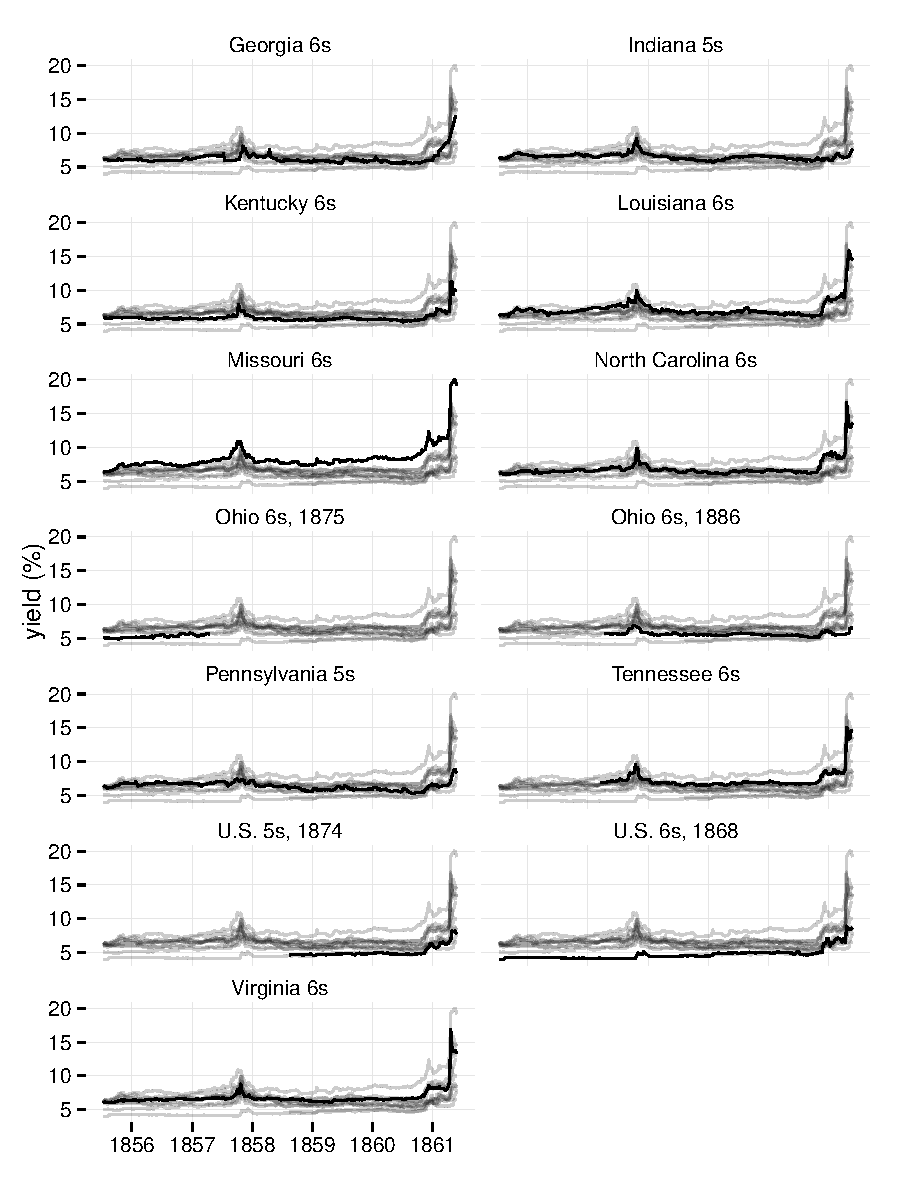
\includegraphics[width=\textwidth]{./figures/fig_yields_all-1}
\caption{Yields on U.S. government and state bonds, July  1, 1855--June  1, 1861}
\label{fig:yields_all}
\end{figure}


\begin{figure}
  \centering
  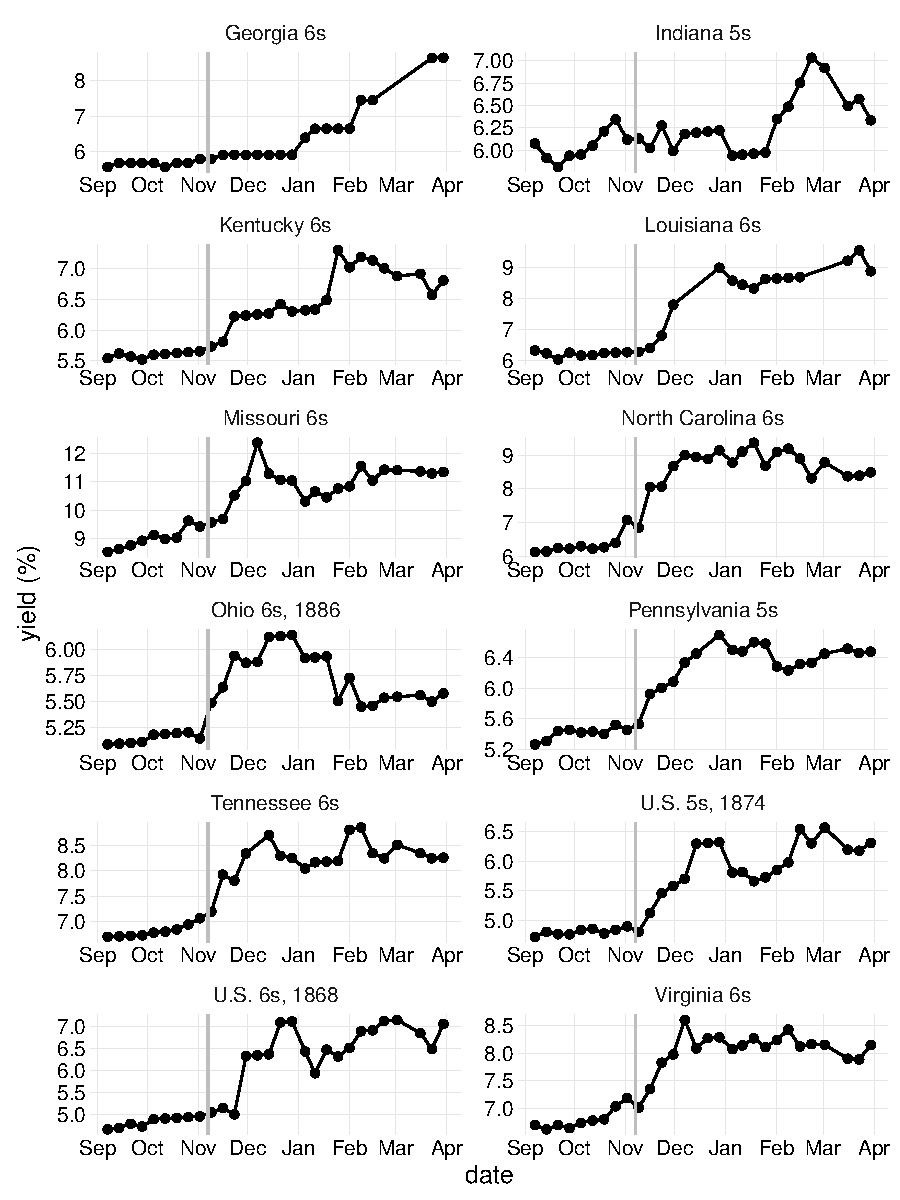
\includegraphics[width=\textwidth]{./figures/fig_yields_election-1}
\caption[Yields on U.S. government and state bonds around the Presidential Election of 1860]{
  Yields on U.S. government and state bonds around the Presidential Election of 1860.
  The vertical lines indicate the date of the election, November 6, 1860.
}
\label{fig:yields_election}
\end{figure}

\begin{figure}
  \centering
  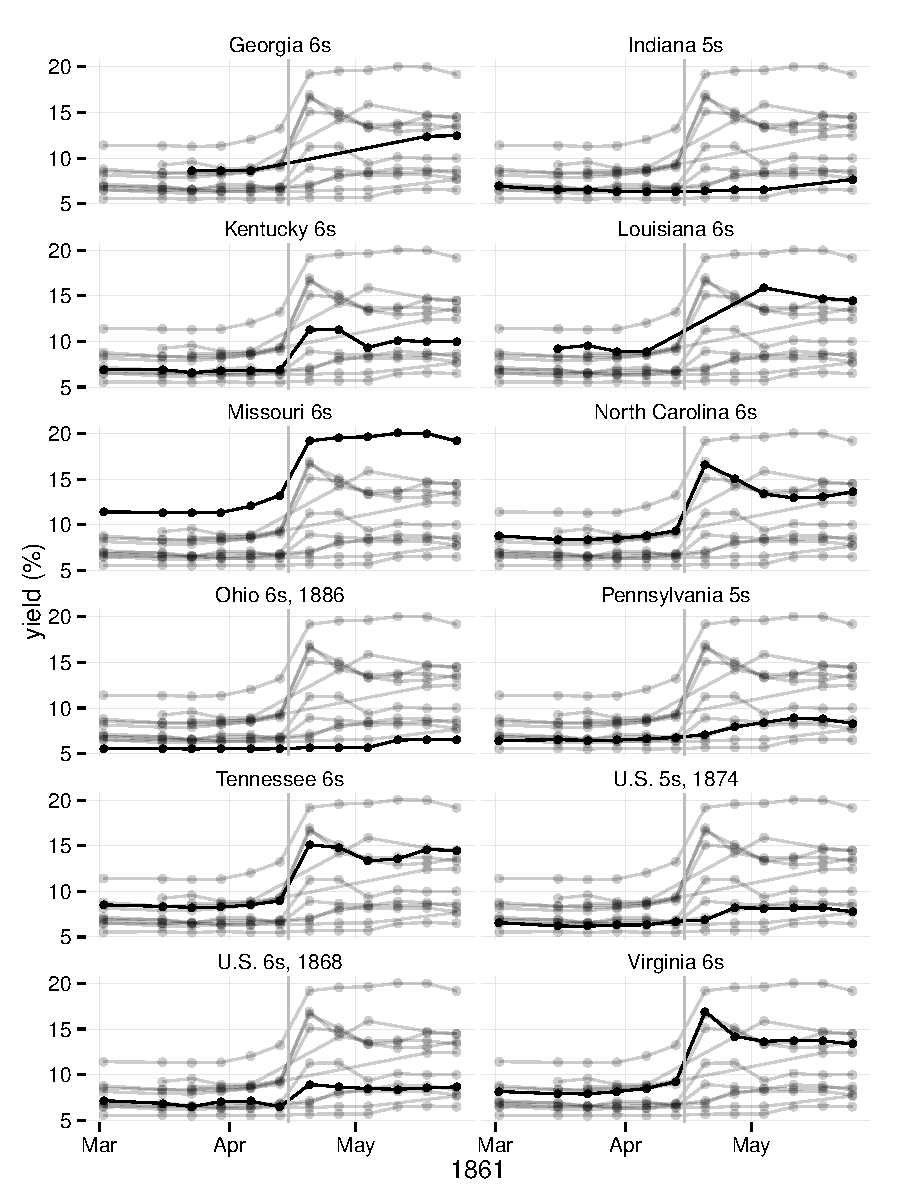
\includegraphics[width=\textwidth]{./figures/fig_yields_sumter-1}
\caption[Yields to maturity of U.S. government and state bonds before and after the Battle of Fort Sumter.]{
  Yields to maturity of U.S. government and state bonds before and after the Battle of Fort Sumter.
  The vertical lines indicate the date when news of the surrender of Fort Sumter reaches New York, April 15, 1861.
}
\label{fig:yields_sumter}
\end{figure}

Figure~\ref{fig:yields_all} plots the yields of all bonds in the data from July  1, 1855 to June  1, 1861, a couple months after the start of the American Civil War.
By visual inspection, these time series can be divided into five periods:
July 1855 to October 1857,
November 1857 to January 1858 (the Panic of 1857),
February 1858 to October 1860,
November 1860 to April 14, 1861 (Battle of Fort Sumter),
and after the Battle of Fort Sumter.



From July 1855 through October 1857, both the level and variance of the yields was low.
The yields of the U.S. Sixes of 1868 were between 3.9 and 4.3\%.
At that time, these were the lowest yields on U.S. government bonds \parencite[282-283]{HomerSylla2005}.
The yields were even lower than the traditionally safe Massachusetts and Boston city bonds, and less than one percent age point higher than the yield on 3\% British consols, which were considered the safest global asset during that period.%
\footnote{The average annual yields on British consols 1855-1857 were between 3.27 and 3.31 \parencite[193]{HomerSylla2005}.}
State bond yields were also relatively stable, although having higher yields than government bonds; with average yields between 5.3 (Ohio 6s, 1875) and 7.6 (Missouri 6s).
State bonds had higher yields than U.S. government because were perceived to be riskier assets.
In particular, in the 1840s nine states or territories defaulted on their debts \parencite{English1996}.%
\footnote{Of the states with bonds in the data, Indiana, Pennsylvania and Louisiana defaulted in the 1840s \parencite[265]{English1996}.}
%Although higher than government bond yields, the yields of the state bonds during this period were still much lower than the previous decade, when some states had yields of above 10\% and as high as 41\% \parencite[320]{HomerSylla2005}.
Overall, the relatively low and stable yields suggest that the market did not assign much, if any, risk to war.
% TODO: discuss Missouri. But would need to do structural break analysis.

Between October 1857 to January 1858, yields spiked during the Panic of 1857.
The Panic of 1857 was a recession and financial crisis that included the failure of a major insurance company, the failures of banks and railroads, and the suspension of specie payments by banks in New York City.
The causes of the panic were not directly related to political risks of secession or war, but were most likely a decline in European demand for U.S. imports or insufficient specie supply to meet demand due to a decline in gold production \parencites[263-265]{Dewey1918}[277,299]{HomerSylla2005}[337]{BankersMagazine1857}.
The \textit{Bankers' Magazine} ``Notes on the Money Market'' sections of the time do not mention domestic political issues during the Panic of 1857, attributing it to a decline in foreign trade and bad banking \parencite[337]{BankersMagazine1857}.
Thus, while yields reached high levels the panic, these high yields are almost certainly not attributable to an increase in war risk.

After the Panic of 1857, from February 1858 to November 1860, yields of bonds returned to levels similar to the period prior to the Panic of 1857.
While the yields of U.S. government bonds were also stable during this period, their yields were approximately 0.5 percentage points higher than they had been before the panic.
The yields of state bonds were also similar to, or in some cases lower than, in the period prior to the panic.

Lincoln's victory in the presidential election on November 6, 1860 precipitated a rise in yields, especially for Southern state bonds.%
\footnote{Lincoln's victory was known the next day: ``It is too certain to speak confidently of detailed results of yesterday's elections. But there can be no reasonable doubt that the Republicans have elected their president.'' \parencite{NYT1860}}
The yields of bonds before and after the election are plotted in Figure~\ref{fig:yields_election}.
The market partially anticipated the political issues that would arise with Lincoln's election, as there was a slight increase in yields in October 1860.
This rise was partially due to a monetary contraction as the economy went into recession \parencite[413]{BankersMagazine1860}, but also the anticipation of a Republican victory in the election.%
\footnote{The United States was in a slight recession prior to the start of the American Civil War, from October 1860 to June 1861, according to the  \href{http://www.nber.org/cycles/cyclesmain.html}{NBER}.}
The \textit{Bankers' Magazine} described the market,
\begin{quote}
   The market for Government and State loans during the month has been dull.
   Prices have in most instances tended downward and a material decline is perceptible in some of the most prominent securities.
   The principal reasons for this seem to be the political excitement.  \parencite[414]{BankersMagazine1860}
\end{quote}
The market reaction was likely in response the Republican victory in the Pennsylvania gubernatorial election on October 9:
\begin{quote}
  The election in Pennsylvania early in October and the prospect which it gave of the election of the Republican candidate for President in November caused the timid to pause. ...
  The political complications of the day were the sole cause relied on by the bears and totally ignoring every other element in the market the pressure to sell under the influence of this sudden fear of some dreadful calamity became irresistible. ...
  The partisan presses aided the decline as far as they could and did their best to make it a panic by spreading abroad the most gloomy picture of the state of feeling at the South and directly prophesying ruin complete and full in the event of Mr. Lincoln's election.
  \parencites[476-77]{BankersMagazine1860}
\end{quote}
While the market believed it was likely that Lincoln would win the election and aware that Lincoln's election cause political risk, the  response observed in the yields was minimal.

It was not until after Lincoln's election that yields increased substantially.
This increase did not occur immediately after Lincoln's election victory.
Instead, yields rose over the course of the following month, with some variation between bonds in the timing of the rise.
However, by the end of January 1861, Southern and border state yields had increased 1--3 percentage points, and the yields on U.S. government bonds had increased 1--1.5 percentage points.
The initial increase in yields was due to a financial crisis that started when Southern banks started denying credit to Northern clients and withdrew their specie from Northern banks \parencite[76]{HomansDana1861a}.
However, while this crisis largely resolved by November \parencite[539-542]{BankersMagazine1860}, the political risk remained:
\begin{quote}
  The money market during December recovered somewhat from the worst effects of the panic.
  The action of the banks had been prompt and energetic, and the relief afforded by their largely expanded line of loans and discounts averted the worst consequences of the panic.
  The want of confidence in the political future prevented however a complete recovery and the results of prostrated credit and destroyed confidence were everywhere discernible. \parencite[December 1860,][541]{BankersMagazine1860}
  The only speck in the horizon is the threat of secession in the South.
  We would be the last to give countenance to the libel upon the South, that the majority of any one State assented to the proposition of secession.
  The permanent social, commercial and financial interest of the various sections of the whole country are too strongly identified---too strongly bound together---to induce the loss of any one State. \parencites[January 1860,][419]{BankersMagazine1860}
\end{quote}
While yields increased during this period, the yields on most bonds were less than their peak during the Panic of 1857.

Yields for many bonds continued rising until the ordinance of secession by South Carolina on December 20, 1860.
In the months between the election and the start of the war, both the level and variance of yields was high as they responded to political events \parencites[718]{HuntKettellHomansEtAl1860}[78,198,416,677]{HomansDana1861a}[413,481,669,756,838]{BankersMagazine1860}.%
Comparing the individual series of the Southern state bonds, the market appeared to have treated Southern states similarly, regardless of whether they had formally seceded prior to the start of the war.
This suggests that few of the secessions came as a surprise.
For example, Louisiana did not secede until January 26, but its yield had already peaked at near 9\% at the start of January.
Virginia, Tennessee and North Carolina did not secede until after Fort Sumter, yet the yields on all of these states rose between November and January.%
\footnote{Georgia is an exception; its yields noticeably increase after the election until January 1861 near is declaration of secession (January 19, 1861).
This may be because the Georgia Sixes were illiquid; in the data, there are long sequences in which the price of the Georgia bonds does not change, and it is often traded in multiples of 5 or 10.
}

Although bond yields had risen after the election of Lincoln and the formation of the Confederate States, the start of the war with the Battle of Fort Sumter (April 12--13, 1861) was followed by a jump in yields much larger than had been observed in the period leading up to the war, or even during the Panic of 1857.
The start of the war resulted in a ``depreciation in Southern State stocks exceeding any decline ever witnessed at the stock board of this city \parencite[919]{BankersMagazine1860}.''
Unlike after the election of 1860, in which bond yields rose over a period of weeks, prices fell and yields rose immediately after the surrender of Fort Sumter.
Figure~\ref{fig:yields_sumter} plots the yields around the Battle of Fort Sumter (March--June 1861).
Table~\ref{fig:yields_sumter} tabulates yields in the week immediately before and after news of the surrender of Fort Sumter reached New York.
Southern state yields rose between 6.1 (Tennessee) and 7.7 (Virginia) percentage points (41 and 45\%) between April 13th and 20th.
The yields of U.S. sixes also rose, but only by 2.5 percentage points,
while Northern state bond yields were almost unchanged.%
\footnote{The price of the U.S. Fives of 1874 did not change noticeably until the following week, April 27, 1861}
Since the yield of the bond incorporates expectations about future payoffs and war would certainly affect those payoffs, the extreme rise in yields after Fort Sumter imply that the probability the market assigned to war was low.
This means that the market most have anticipated some sort of peaceful settlement to the crisis short of war.
In April 1861, \textit{The Bankers' Magazine} wrote, ``The general condition of commercial and financial affairs still turns upon the uncertain political future. The fears of civil war, that at one time were entertained in certain quarters, have subsided, if not altogether disappeared, under the influence of passing events \parencite[413]{HomansDana1861a}''
while \textit{The Merchants' Magazine} wrote,
\begin{quotation}
  The securities of the Border States fluctuate from day to day as the tone of dispatches from Washington leans toward peace or war.
  There is undoubtedly a great want of confidence as to the final course which those States will pursue and it is the strong hope which is entertained of their remaining loyal which alone keeps up their price. \parencite[838]{BankersMagazine1860}
\end{quotation}
The speed and size of the reaction of bonds yields after the Battle of Fort Sumter implies that the market's hope that Southern states would remain loyal must have been strong, and it was surprised that the political crisis had escalated into war.
The reaction of the market to the Battle of Fort Sumter also implies that the market considered this the start of major hostilities, even though large-scale engagements would not occur until months later with the First Battle of Bull Run.

\section{South-North Yield Spread}
\label{sec:south-north-yield}


\begin{figure}
  \centering
  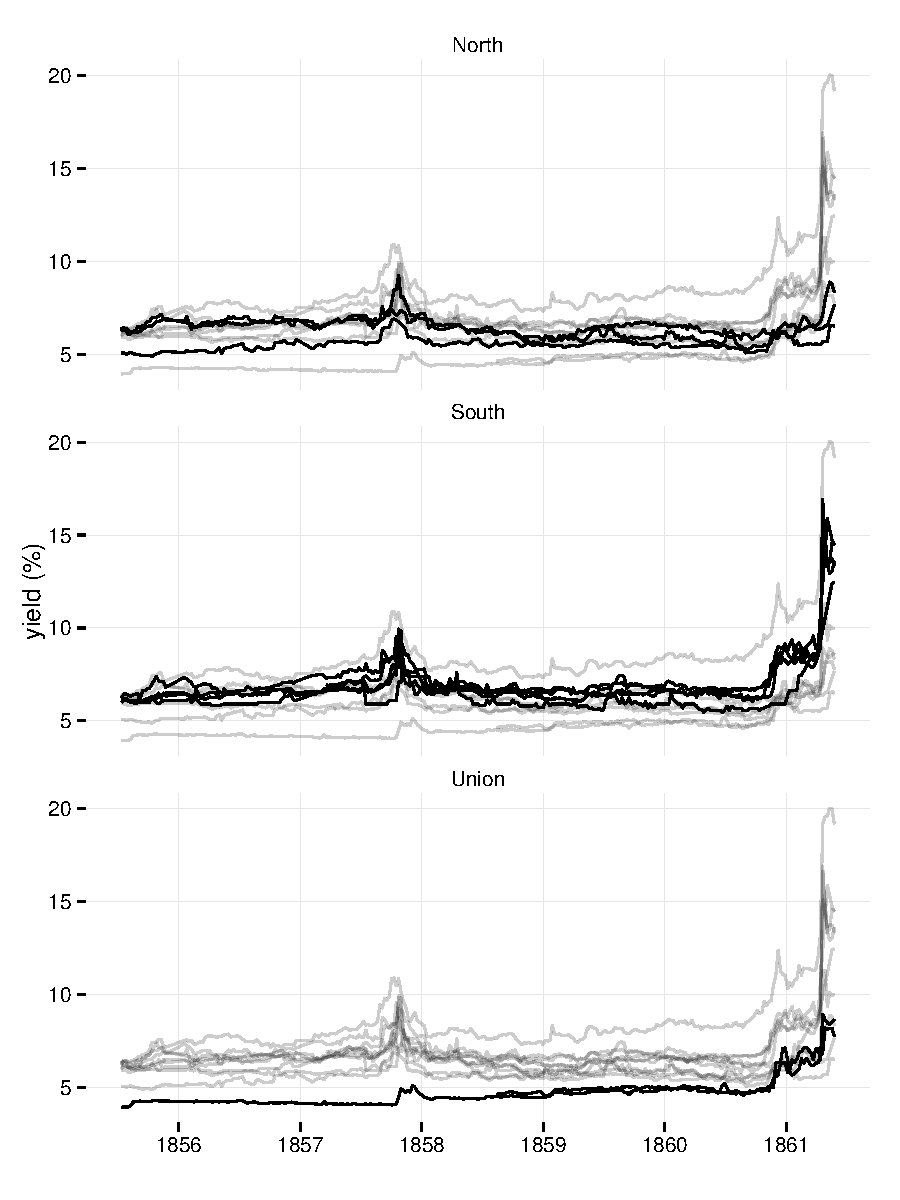
\includegraphics[width=\textwidth]{./figures/fig_yields_regions-1}
\caption{Yields of U.S. government and state bonds, by region, July  1, 1855 to June  1, 1861.}
\label{fig:yields_regions}
\end{figure}

\begin{figure}
  \centering
  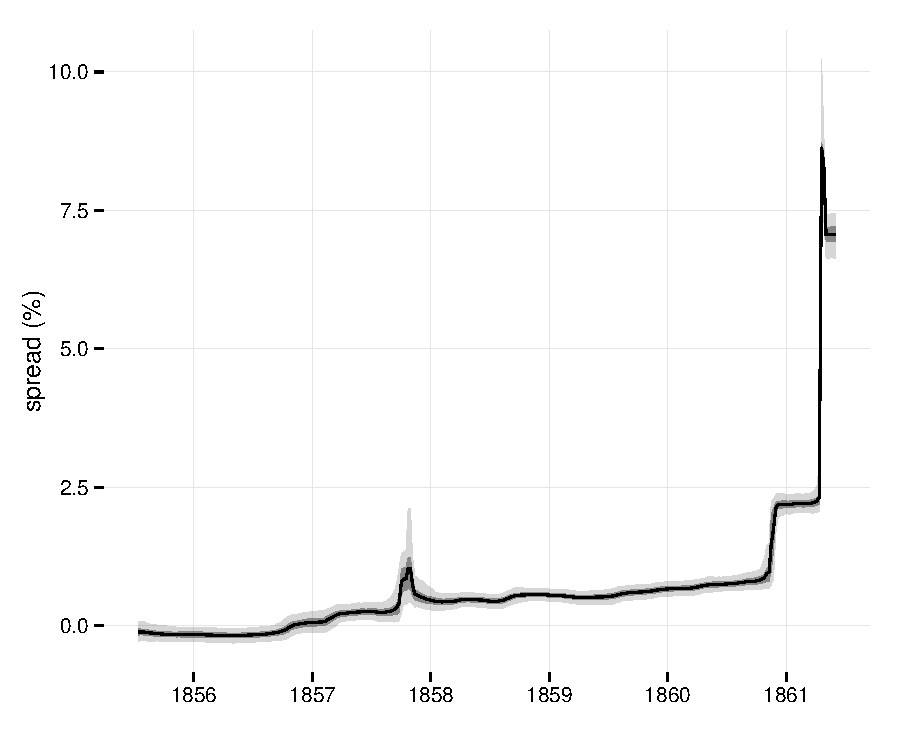
\includegraphics[width=\textwidth]{./figures/fig_north_south_spreads-1}
\caption[Yield spread between Southern and Northern state bonds]{
  Yield spread between Southern and Northern state bonds.
  The line is the posterior mean, the dark ribbon is the 50\% credible interval, the light ribbon is the 95\% credible interval.
}
\label{fig:north_south_spreads}
\end{figure}

For the case of the American Civil War, the spread between the yields of the Southern and Northern state bonds measures the difference in risk between these bonds, and a measure of war risk.%
\footnote{
  The spread between Southern and Northern bonds is approximately the difference in default risk between the bonds, when the recovery rate is 0.
  This follows from Equation~\eqref{eq:4}.
}
An increased risk of war increases the spread would make Southern state bonds relatively more risky than Northern state bonds.
Although war could increase the riskiness of all state bonds, there are at least two reasons why a war would increase the risk of Southern state bonds relative to Northern state bonds.
First, Southern states would stop the payment of interest to Northern investors in the event of a war.
As discussed in Section~\ref{sec:risky-bond-pricing}, the suspension of interest did happen and was anticipated by investors.
Second, it is likely that a war would be fought primarily in Southern states, and Southern states would incur more costs which could hinder their ability to repay debt in the future.%
\footnote{In the estimates of the economic cost of the American Civil War in \textcite{GoldinLewis1975}, physical capital loss was the largest component of the direct cost of the war to the Confederacy \parencite[308]{GoldinLewis1975}}
The differential effect the war on the risk of Southern and Northern bonds was observed in the changes in the yields of these bonds after the Battle of Fort Sumter, as shown in Table~\ref{tab:sumter}.
In the week after after Fort Sumter, the yields of Southern states increased 3--8 percentage points, while the yields of Northern states increased by less than one percentage point.
An advantage of using the spread rather than the yields of each bond, is that it controls for shocks which affect all state bonds.
While there could be other non-war regional factors that accounted for the spread between Southern and Northern state bonds, using the change in the spread controls for any constant regional factors.

The data used to calculate the south-north yield spread consist of the yields of Northern state bonds (Indiana, Ohio and Pennsylvania) and Southern state bonds (Georgia, Louisiana, North Carolina, Tennessee and Virginia).
\footnote{The border states of Kentucky and Missouri are not included in these calculations.}
Let $y_{j,t}$ be the yield for bond $j$ at time $t$.
The yield for each bond is modeled as,
\begin{equation}
  y_{j,t} \sim \dt{\nu}{\theta_{t} + \psi_{t} \mathtt{south}_{j}, \sigma} \text{,}
\end{equation}
where $\dt{a}{b, c}$ is the Student's $t$-distribution with degrees of freedom $a$, location $b$ and scale $c$, and
$\mathtt{south_{j}}$ is a binary variable indicating whether bond $j$ was issued by a Southern state.

Since the number of bonds in each period is relatively small, the parameters $\theta$ and $\psi$ are smoothed over time with random walk priors.
However, the method used to pool rates over time cannot overly smooth the data since the method would obscure the effect of important events on the spread.
In order to achieve behavior similar to a change-point model, this work uses a shrinkage prior for the first difference of $\psi$ and $\eta$,
\begin{align}
  \theta_{t} & \sim \dnorm{\theta_{t-1}, \sigma^{2} \tau_{\theta}^{2} \lambda_{\theta,t}^{2}}
  & \lambda_{\theta,t} & \sim \dhalfcauchy{0, 1} \text{,} \\
  \psi_{t} & \sim \dnorm{\psi_{t-1}, \sigma^{2} \tau_{\psi}^{2} \lambda_{\psi,t}^{2}}
  & \lambda_{\psi,t} & \sim \dhalfcauchy{0, 1} \text{,}
\end{align}
where $\dnorm{a, b^{2}}$ is the normal distribution with mean $a$ and scale $b$, and $\dhalfcauchy{0, a}$ is the half-Cauchy distribution with scale $a$.%
Shrinkage priors are the Bayesian equivalent to penalized estimate like lasso \parencites{Tibshirani1996}{ParkCasella2008}.
The particular shrinkage prior employed horseshoe prior distribution is used \parencites{CarvalhoPolsonScott2009}{CarvalhoPolsonScott2009}.
Although a continuous distribution, the horseshoe prior has properties similar to a spike-and-slab prior.%
\footnote{This approach is similar to a Bayesian version of the fused lasso \textcite{TibshiraniEtAl2005} using the horseshoe prior distribution rather than a Laplace distribution for the reasons discussed in \parencites{CarvalhoPolsonScott2009}{CarvalhoPolsonScott2009}.}
\footnote{Note that variable and parameter names are only unique for this section; variables and parameters with the same name in different sections do not necessarily correspond to the same thing.}
In summary, this set of priors method attempts to estimate the parameters, e.g. $\theta$, where the first differences, $\theta_{t} - \theta_{t-1}$, are sparse (mostly zero) while not imposing assumptions about the sparsity of the differences.
The posterior distribution of this model is sampled with the HMC No-U-Turn Sampler implemented in Stan \parencites{Stan2014}{HoffmanGelman2014a}.

Figure \ref{fig:north_south_spreads} plots estimates from the posterior distribution of the south-north spread ($\psi_{t}$) for all periods.
For most periods, the spread was positive, meaning that Southern state bonds were riskier than Northern state bonds on average.
The spread is increasing over most of the period before stabilizing before the presidential election
Between the start of the period (July 1, 1855) and the presidential election of 1860 (November 2, 1860), the spread increased by 1.06 (0.73, 1.45),
from -0.11 (-0.28, 0.08) to 0.95 (0.68, 1.45).
The spread increased even though the yields of Southern bonds remained largely stable or even slightly declined, because the yields of Northern bonds, especially Indiana and Pennsylvania, declined by more.
The Panic of 1857 had some effect on the spread, but less than for the yields, and the uncertainty in the estimated spread increases during that period.
The spread increases sharply after the election of Lincoln, increasing by 1.23 (0.7, 2.4) percentage points to 2.18 (1.95, 2.4) on December 7, 1860.
The spread is stable until the the Battle of Fort Sumter, when it increases 6.31 (5.47, 7.88) percentage points to 2.32 (2.07, 2.91).

Thus the risk of Southern bonds relative to Northern bonds was increasing over the period, perhaps due to increasing assessments of the risk of war.
The market's beliefs about the risk of war jumps after Lincoln's election, but the jump in spreads is about 5 times smaller than the spread that is observed after the start of the war.

\section{Probability of War}
\label{sec:probability-war}


While the bond yields and spreads between Northern and Southern bonds can indicate changes in war risk, they are not directly interpretable as the probability of war.
However, the market's beliefs about the probability of war can be inferred from bond prices and yields by treating war as a default event.%
\footnote{
  \textcite{HaberMitchenerOosterlinckEtAl2015} use a similar method by treating loss in war as a default event. 
  See \textcites{Fons1987}{Merrick2001}{Chan-Lau2006} for derivations of default probabilities from bond prices.
}
A simple approximation for the probability of risk-neutral default probability per year of a risky bond given its yield is,
\begin{equation}
  \label{eq:4}
  \Pr(\text{default}) = \frac{y - r}{1 - R} \text{,}
\end{equation}
where $y$ is the yield of the risky bond, $r$ is the yield of a risk-free bond with comparable cash flows, and $R$ is the the recovery value of the bond in the event of the default as a proportion of the face value of the bond \parencite{HullPredescuWhite2004}.%
\footnote{\textcite[115]{WaldenstromFrey2008} propose a similar method, that when the war is observed the probability of war is the proportion of the yield after war to the yield prior to war.
  That method is not directly derived from a cash flow model and produces higher estimates of the probability of war.
  \textcite{HaberMitchenerOosterlinckEtAl2015} use a cash flow method to calculate the probability of victory in wars (Confederate victory in the American Civil War, and government victory in the Chinese Civil War) using a cash flow pricing model of bonds, but assuming a recovery rate of 0.
}
Equation~\eqref{eq:4} can be used to estimate the probability of war if $r$ and $R$ are properly defined.

When estimating the probability of war, the risk-free interest rate, $r$, should be defined to be the yield of a comparable bond with no risk of war.
In this case, $r$ will not necessarily be risk-free; the war risk-free should exclude risk due to war, but include any non-war risks.
For $r$, this work will use the average yield of the same bond for an earlier period in which the risk of war is negligible.

The recovery rate, $R$, is the amount as a proportion of par value that the investor receives in the event of a war.
If war does occur, then the value of $R$ to use is straightforward because it is known --- it is the price of the bond observed at the start of the war.
The implied probability of war is calculated for all Southern and Border state bonds: Georgia, Kentucky, Louisiana, Missouri, Tennessee, and Virginia.
For each bond $j$, the implied probability of war, $\pi_{t}$, is
\begin{equation}
  \pi_{t} = \frac{y_{j,t} - r_{j}}{1 - R_{j,t}} \text{.}
\end{equation}
For each bond, $r_{j}$ is its average yield for the period prior to the Panic of 1857, July  1, 1855 to September  1, 1857.
Although there may have been some risk of war during this period, the level of yields were low, and thus war risk could not have been high, as discussed in Section~\ref{sec:data}.
While this estimate of the war-risk free rate accounts for the risk heterogeneity between the bonds, it makes the strong assumption that $r_{j}$ is that it is constant over time.
Since it does not allow the war-risk free rate to vary over time, the estimates of the probability of war can be confounded by any factors which affect $r$.
In order to reduce this possibility, I only consider the period between the Panic of 1857 and the Battle of Fort Sumter, when there are no major non-war financial crises and changes in war risk are most likely.

For each bond, the value of $R_{j,t}$ is the price of the bond immediately after the start of the war.
More precisely, $R_{j,t}$ is the present value of bond $j$ at time $t$ calculated using the average yield of the bond April 15, 1861 to May 18, 1861.%
\footnote{
  If the first price after Fort Sumter were used, the implied probabilities would be even higher than those reported here since yields spiked in the week after Fort Sumter.
}
The value of $R_{j}$ incorporates expectations about the financial risk posed by expected course of the war, which is key to allowing separating the war-risk due to the probability of war and the risk due to the expected costs of the war, conditional on the war occurring.%
\footnote{
  An implicit assumption in these calculations is that expectations about the costliness of the war were constant prior to the start of the war and only beliefs about the probability of a war was changing prior to the war.
  In the case of the American Civil War, this seems like a reasonable assumption.
}

Figure~\ref{fig:prwar1} displays the implied probabilities of war for each bond calculated with Equation~\eqref{eq:4}.
There are three things to note about the implied probabilities in that figure.
First, the implied probability of war is approximately 0 for all bonds prior to the election of Lincoln in 1860.
Second, although the implied probabilities increase after the election, they only increase to between 3 and 5\%.
Third, although there are differences in the probability of war implied by each bond, they largely agree.

The estimate of the implied probability of war can be improved by noting that the implied probability of war should be the same for all bonds.
By rearranging Equation~\eqref{eq:4} and adding an error term, the probability of war in each time period can be estimated as,
\begin{align}
  \label{eq:1}
  \log y_{j,t} & \sim \dnorm{(1 - R_{j}) \pi_{t} + r_{j}, \sigma^{2}} \text{,}
\end{align}
where $\pi_{t}$ is the probability of war at time $t$.
Equation~\eqref{eq:1} is a regression model with time-varying coefficients ($\pi_{t}$).
The inverse logit transformation of $\pi$ evolves as a random walk with a horseshoe prior on the innovations to allow for jumps in its level, \textit{i.e.} change-points, as described in Section~\ref{sec:south-north-yield}:
\begin{align}
  \pi_{t} &= \logit^{-1}(\theta_{t}) \text{,} \\
  \phi_{t} &\sim \dnorm{\phi_{t-1}, \tau^{2} \lambda_{t}^{2}} \text{,} \\
  \lambda_{t} &\sim \dhalfcauchy{0, 1} \text{.}
\end{align}
%% Since the war-risk free interest rate of the bonds are uncertain:
%% \begin{align}
%%   r_{j} & \sim \dnorm{\bar{r}_{j},s_{j}}
%% \end{align}
%% where $\bar{r}_{j}$, $s_{j}$ are the mean and standard deviation of the logarithm of yields for bond $j$ for the period, DATEFMT_PEACE_START  to DATEFMT_PEACE_END.
The estimated values of $\pi_{t}$ from this model are plotted in Figure~\ref{fig:prwar2}.
This model estimates the probability of war to be approximately zero prior to Lincoln's election.
After the election, the probability of war rose to 2.5 (2.1, 2.8)\% by January 5, 1861,
to 3 (2.6, 3.4)\% on February 8, and to 4.1 (3.3, 4.9) on April 13, days before news of the outcome of the Battle of Fort Sumter reached the market.

These results are consistent with the results in Section~\ref{sec:south-north-yield}.
Prior to the election of Lincoln, the market estimated that war would almost certainly not occur.
Only after the election did the market adjust its estimates of the risk of war upwards, however it still considered war to be unlikely.
Even the week before the war, the probability of war was estimated to be highly unlikely.
The results differ in that although both measures show little risk of war prior to the election of Lincoln, the estimates of south-north yield spread show an increasing risk of war over time, while the implied probability of war from this section show that risk constant at nearly zero.
This difference likely arises from the use of a constant war-risk free rate in Equation~\eqref{eq:1}.%
\footnote{
  This could be avoided if a good time-varying estimate of the war-risk free interest rate were available.
  Currently available data of the risk free interest rate of the era are only available at low frequencies: prior to 1857, the yields of Massachusetts Fives and Boston City bonds are only available at a yearly frequency prior; after 1857, an index of New England state and municipal bonds is available at a quarterly frequency \parencite{Officer2003}.
  Using the average of Northern state bonds, as in Section~\ref{sec:south-north-yield}, is likely inappropriate because they also include some risk of war.
}

\begin{figure}
  \centering
  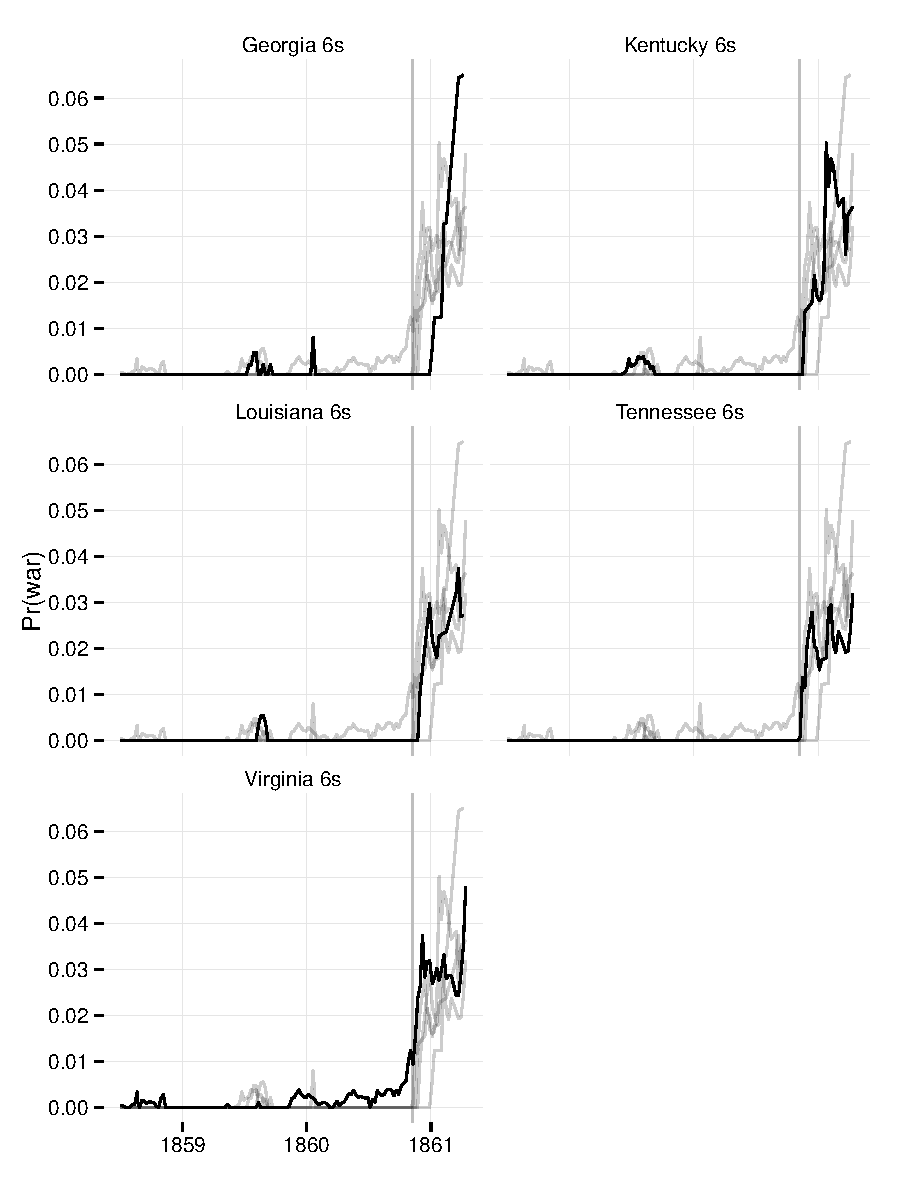
\includegraphics[width=\textwidth]{./figures/fig_prwar1-1}
  \caption{Implied probabilities of the initiation of war calculated from each Southern and Border state bond, March  5, 1858 to April 13, 1861.}
  \label{fig:prwar1}
\end{figure}

\begin{figure}
  \centering
  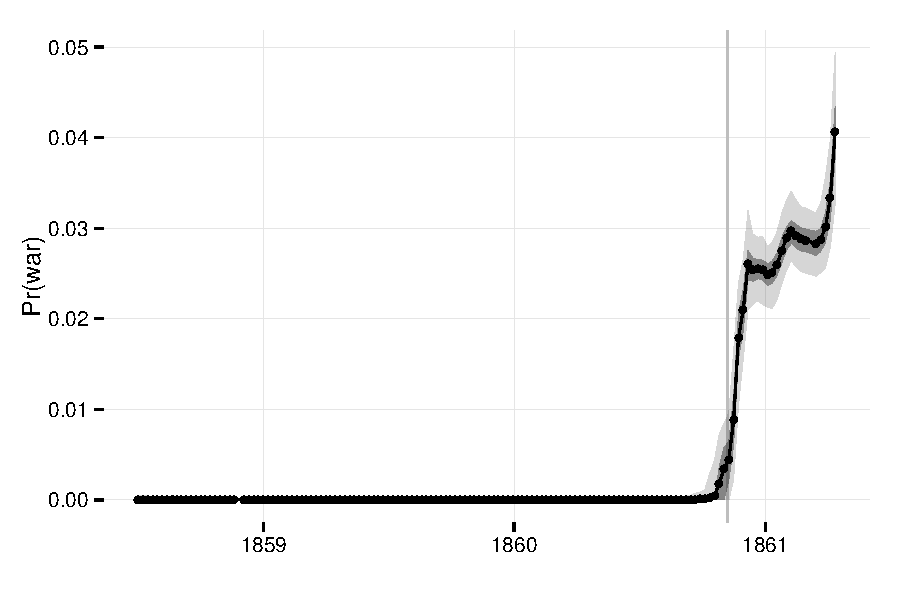
\includegraphics[width=\textwidth]{./figures/fig_prwar2-1}
  \caption[Implied probabilities of the initiation of war calculated from a latent variable model of the prices U.S. government and Southern and border state bonds, March  5, 1858 to April 13, 1861, using the model described in section \ref{sec:probability-war}]{
    Implied probabilities of the initiation of war calculated from a latent variable model of the prices U.S. government and Southern and Border state bonds, March  5, 1858 to April 13, 1861, using the model described in section \ref{sec:probability-war}.
    The line is the posterior mean, the dark ribbon is the 50\% credible interval, the light ribbon is the 95\% credible interval.
    The vertical line is the date of Abraham Lincoln's election.
  }
  \label{fig:prwar2}
\end{figure}

\begin{table}
  \centering
  % latex table generated in R 3.2.2 by xtable 1.7-4 package
% Mon Oct 19 12:58:41 2015
\begin{tabular}{rrrrr}
  \hline
 & \parbox{2.5cm}{\raggedleft Avg. yield \\ 1858-02-01--\\1860-11-07} & \parbox{2.5cm}{\raggedleft Avg. yield \\ 1860-11-07--\\1861-04-15} & \parbox{2.5cm}{\raggedleft $r$\\ Avg. yield \\ 1855-07-01--\\1857-09-01} & \parbox{2.5cm}{\raggedleft $R \cdot 100$ \\ Avg. price \\ 1861-04-15--\\1861-05-18} \\ 
  \hline
Georgia 6s & 5.92 & 6.72 & 6.15 & 62.52 \\ 
  Kentucky 6s & 5.68 & 6.59 & 5.86 & 74.60 \\ 
  Louisiana 6s & 6.70 & 8.31 & 6.90 & 48.00 \\ 
  Tennessee 6s & 6.76 & 8.30 & 7.13 & 43.85 \\ 
  Virginia 6s & 6.50 & 8.12 & 6.48 & 43.65 \\ 
   \hline
\end{tabular}

  \caption{Summary of data used to calculate the probability of war initiation.}
\label{tab:prwar1}
\end{table}

\section{Conclusion}
\label{sec:conclusion}

Although the seeds of the American Civil War preceded the start of the war for many years, the onset of war was surprising to financial markets.
Financial markets did not price in any risk of war until after the election of Lincoln in November 1860. 
Despite awareness of the risk of war, including the secession of several states, yields jumped after the Battle of Fort Sumter, implying that the event was unanticipated.
The implied probability of war based off the Southern state bonds was only about 5\%.

The results presented here are specific to the case of the American Civil War, but they are consistent with other work on how financial markets have responded to war initiation.
\textcite{Ferguson2006} show that although World War I was preceded by a series of crises, European markets did not anticipate its onset.
\textcite{FreyKucher2000} and \textcite{WaldenstromFrey2008} show that Nordic and Swiss markets had large reactions to the start of World War II.
\textcite{GuidolinLaFerrara2010} find large abnormal returns at MIDs.
Many of those works emphasize the efficiency of markets in responding to political events, or use the size of the market reaction to understand characteristics of the political events.
However, the presence of strong market reactions to these events is itself interesting, as it is an indication that the onset of hostilities was unexpected.
Overall, these cases suggest that financial markets may systematically underestimate the risk of war.
There are two interpretations of this.
First, if markets are efficient and incorporate public information, many wars are not anticipated given the information at the time.
Second, markets do a poor job of assessing the \textit{ex ante} theory of war.
Either of these scenarios has important implications for prominent theories of war.

The \textit{ex ante} public information assessments of the probability of war are important because they may provide a method for distinguishing between rationalist theories of war.
The two rationalist theories of war, commitment problems and private information \parencites{Fearon1995,Powell2006}, have different implications as to what the \textit{ex ante} probability of war occurring will be.
Namely, private information model of war implies that wars should be unanticipated \parencite{Gartzke1999}.
Since with a commitment problem wars can occur with complete information, they can be anticipated.
Thus, prevalence of unanticipated wars provides evidence for private information models of war.
Other more specific theories of war may offer different implications as to what the \textit{ex ante} probability of war would be.
However, since theories of war may differ in their implications for the predictability of war, and financial markets provide a means of measuring the predictability of war, financial market data provide another way to test theories of war.
In the specific case here, the low probability of war implied by financial markets for the American Civil War is surprising given that several political science treatments of the American Civil War emphasize commitment problems \parencites{Reiter2009}{Weingast1998}{Poast2012}.
The second possibility is that financial markets maybe doing a poor job assessing and signaling the risk of war.
This would pose serious questions as to the ability of markets to signal prices to the potential belligerents, as in the \textit{capitalist peace}.

% Bibtex commands go here
\printbibliography{}

\end{document}

%% LocalWords:  prwar Fearon1995 GartzkeLiEtAl2001a GartzkeLi2003 
%%  LocalWords:  Reiter2003 Reiter2009 Schwab1901 Mitchell1903 MIDs
%%  LocalWords:  HaberMitchenerOosterlinckEtAl2015 McCandless1996 csv
%%  LocalWords:  WillardGuinnaneEtAl1996 SmithSmith1997 Bueno1990 Sixes
%%  LocalWords:  BrownBurdekin2000 Weidenmier2002 Hall2004 Herron2000
%%  LocalWords:  Ferguson2006 WaldenstromFrey2008 RigobonSack2005 Fives
%%  LocalWords:  SchneiderTroeger2006 GuidolinLaFerrara2010 Elder1865
%%  LocalWords:  heteroskedasticity LeighWolfersEtAl2003 investors'
%%  LocalWords:  WolfersZitzewitz2009 Jayachandr2006 Elder1863 years'
%%  LocalWords:  Merchants' HomansDana1861a Treasury1861a Bankers' 5s
%%  LocalWords:  Treasury1860 Treasury1863 BankersMagazine1860 bdy
%%  LocalWords:  BankersMagazine1862 Randolph1931 Ratchford1941 Pre
%%  LocalWords:  DwyerHaferWeber1999 metadata HomerSylla2005 ytm pre
%%  LocalWords:  DeKnight1900 Martin1871 Macaulay1938 Officer2003 fmt
%%  LocalWords:  English1996 Dewey1918 BankersMagazine1857 NBER diff
%%  LocalWords:  HuntKettellHomansEtAl1860 GoldinLewis1975 Stan2014
%%  LocalWords:  Tibshirani1996 ParkCasella2008 TibshiraniEtAl2005
%%  LocalWords:  CarvalhoPolsonScott2009 HoffmanGelman2013 elec Sixes
%%  LocalWords:  preelec postelec sumter postsumter Fons1987 Fives
%%  LocalWords:  Merrick2001 Lau2006 HullPredescuWhite2004 DATEFMT
%%  LocalWords:  PRWAR1 FreyKucher2000 Powell2006 Gartzke1999 Fives
%%  LocalWords:  Weingast1998 Poast2012 Powell2007 HoffmanGelman2014a
%  LocalWords:  5's 6's HMC
